
Biochemistry and Molecular biology are currently one of the scientific fields, with the largest progress

Fundamental concepts of biochemical concepts the structure of DNA \cite{Watson1953} (with the unpublished work of Rosalind Franklin), the central dogma of Molecular biology \cite{Crick1970},  

Tools: sequencing, CRISPER \cite{Deltcheva2011}, structural BIo
Diseases: like the characterization of cancer \cite{Hanahan2000, Hanahan2011} 


%Structural Biology
With the large advances in structural biology starting from the structure of myoglobin\cite{kendrew1958} and the structure of an $\alpha$-helix \cite{pauling1951}, a new understanding of Biochemistry developed in the last century. \cite{Shi2014}

% MD sims with biochem. first applications
However often in the early perspective proteins were considered to be relatively rigid. This believe was adapted to a much more dynamic understanding of protein structures influenced by methods like Molecular dynamics simulations (MD). \cite{Karplus2002, phillips1981} And later on by developments of experimental methodology, like b-factor, NMR and CryoEM
The first MD simulation shaking contributing to the transition of understanding was performed on the pancreatic trypsin inhibitor (BPTI) for  $9.2~ps$ in vacuum . \cite{McCammon1977} 

%Examples of application
In the past MD was used for many different biological models containing proteins, RNA or DNA, and lipid membranes. 
the first interest was focussing on the sampling of the configuration space at equilibrium under certain physical conditions in order to study the conformational behavior of the molecules, often supported by experiment either directly or indirect as validation. Or to extract thermodynamics  One example of a study of such biochemical interest can be found in \ref{ch:cycPep}
Simulations each now the magnitude of $\mu s$

With the first free energy calculation by \textit{Jorgensen} MD simulations entered the next level of applications.

An additional aspect of applications is drug design.  \cite{Cournia2017, Cournia2020, Jorgensen1983}
Which also has industry use! \cite{Christ2014, Meier2021, Cournia2017, Cournia2020}
But not only free energies are subject of drug design, permeability of possible drug candidates can be a meter. \cite{wang, Witek2016b, Witek2017}


\section{Simulations}
Simulations are powerful tools that allow us to study problems with an underlying model. In copmutational chemistry these models can be based on different layers of theory, like electrons (QM), atoms (MD), or molecules (coarse grained). In this thesis, the theory level of choice was usually atomistic with the united atoms approach. Besides the model representation does a simulation consist of three additional parts: 

%%%Force Field
\subsubsection{Force Fields}
The force field function is used to describe the potential energy $V$ of a given coordinate set of a molecule or system $\vec{r}(t)$. The potential energy landscape (PES) defined by a Force Field function is explored/sampled during a simulation by integrating over time. This process is giving insights in the possible conformations of molecules by the exploration of PES minima. Typical empirical force fields use the sum of all relevant potential energy terms to calculate $V(r)$:
\begin{equation}
    V = V^{bonded} + V^{nonbonded} 
\end{equation}

All force field terms are considered to be relevant for describing the behavior/likelihood of the system in a certain coordinate states. Many force fields functions and parameter sets were developed in the past, like for example: AMBER\cite{}, GROMOS\cite{}, CHARMM\cite{}.

For the thesis we mainly used the GROMOS54A7 force field , the different subterms were defined as follows. 
The bonded potential term consists of 3 sub terms:
\begin{equation}
   V^{bonded} = V^{bond} + V^{angle} + V^{torsion}  
\end{equation}

The bond term  $V^{bond}$ and the angle term $V^{angle}$ were defined as harmonic oscillator \cite{}
\begin{equation}
    V^{bond/angle}~=~\frac{1}{2} k (r-r_0)^2 \\
\end{equation}
\begin{figure}[h]
    \centering
    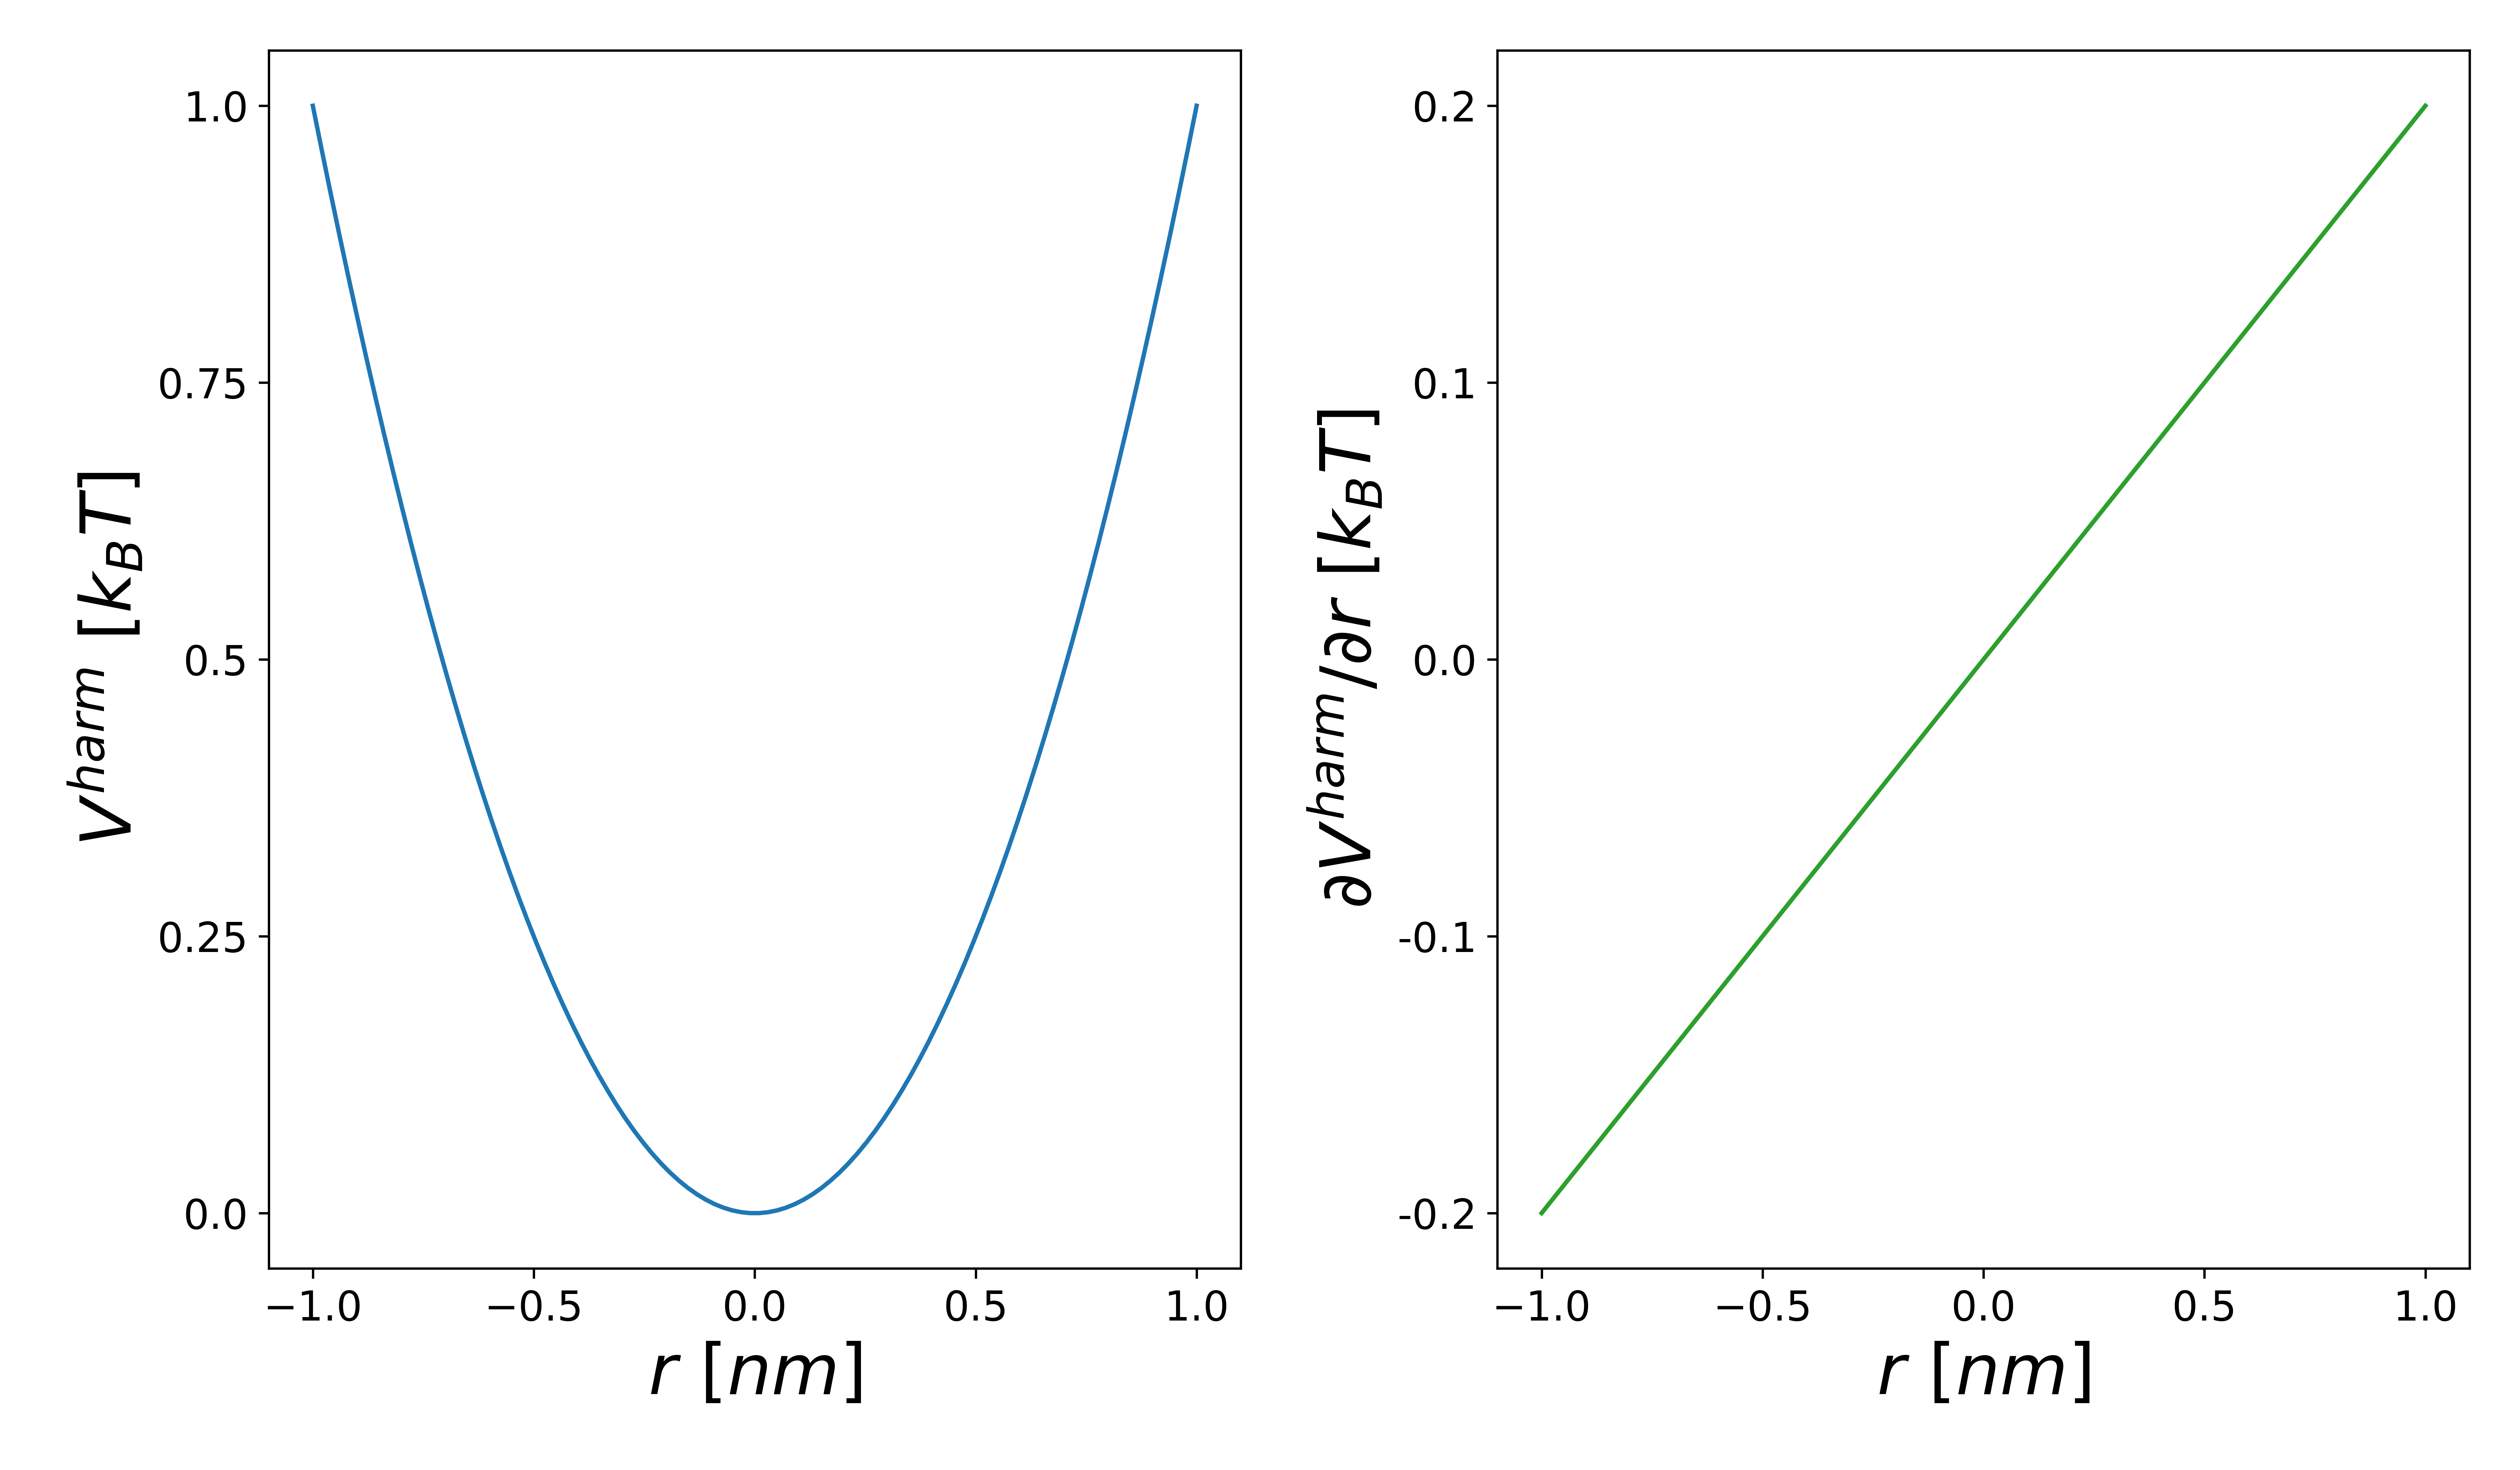
\includegraphics[width=\textwidth]{fig/ForceField/harm_osc.png}
    \caption{Harmonic Oscilator is a standard potential used for bond or angle bending in force fields}
    \label{fig:harmOsc}
\end{figure}

In practice the bond term was neglected to the standardly application of the SHAKE algorithm, that additionally allows a faster time step time of 2fs instead of 1fs.
The torsion dihedral roation term is defined as: 
\begin{equation}
    V^{torsion}~=~\frac{1}{2} k^{torsion}(1+cos(d)cos(m\theta)) \\
\end{equation}
\begin{figure}[h]
    \centering
    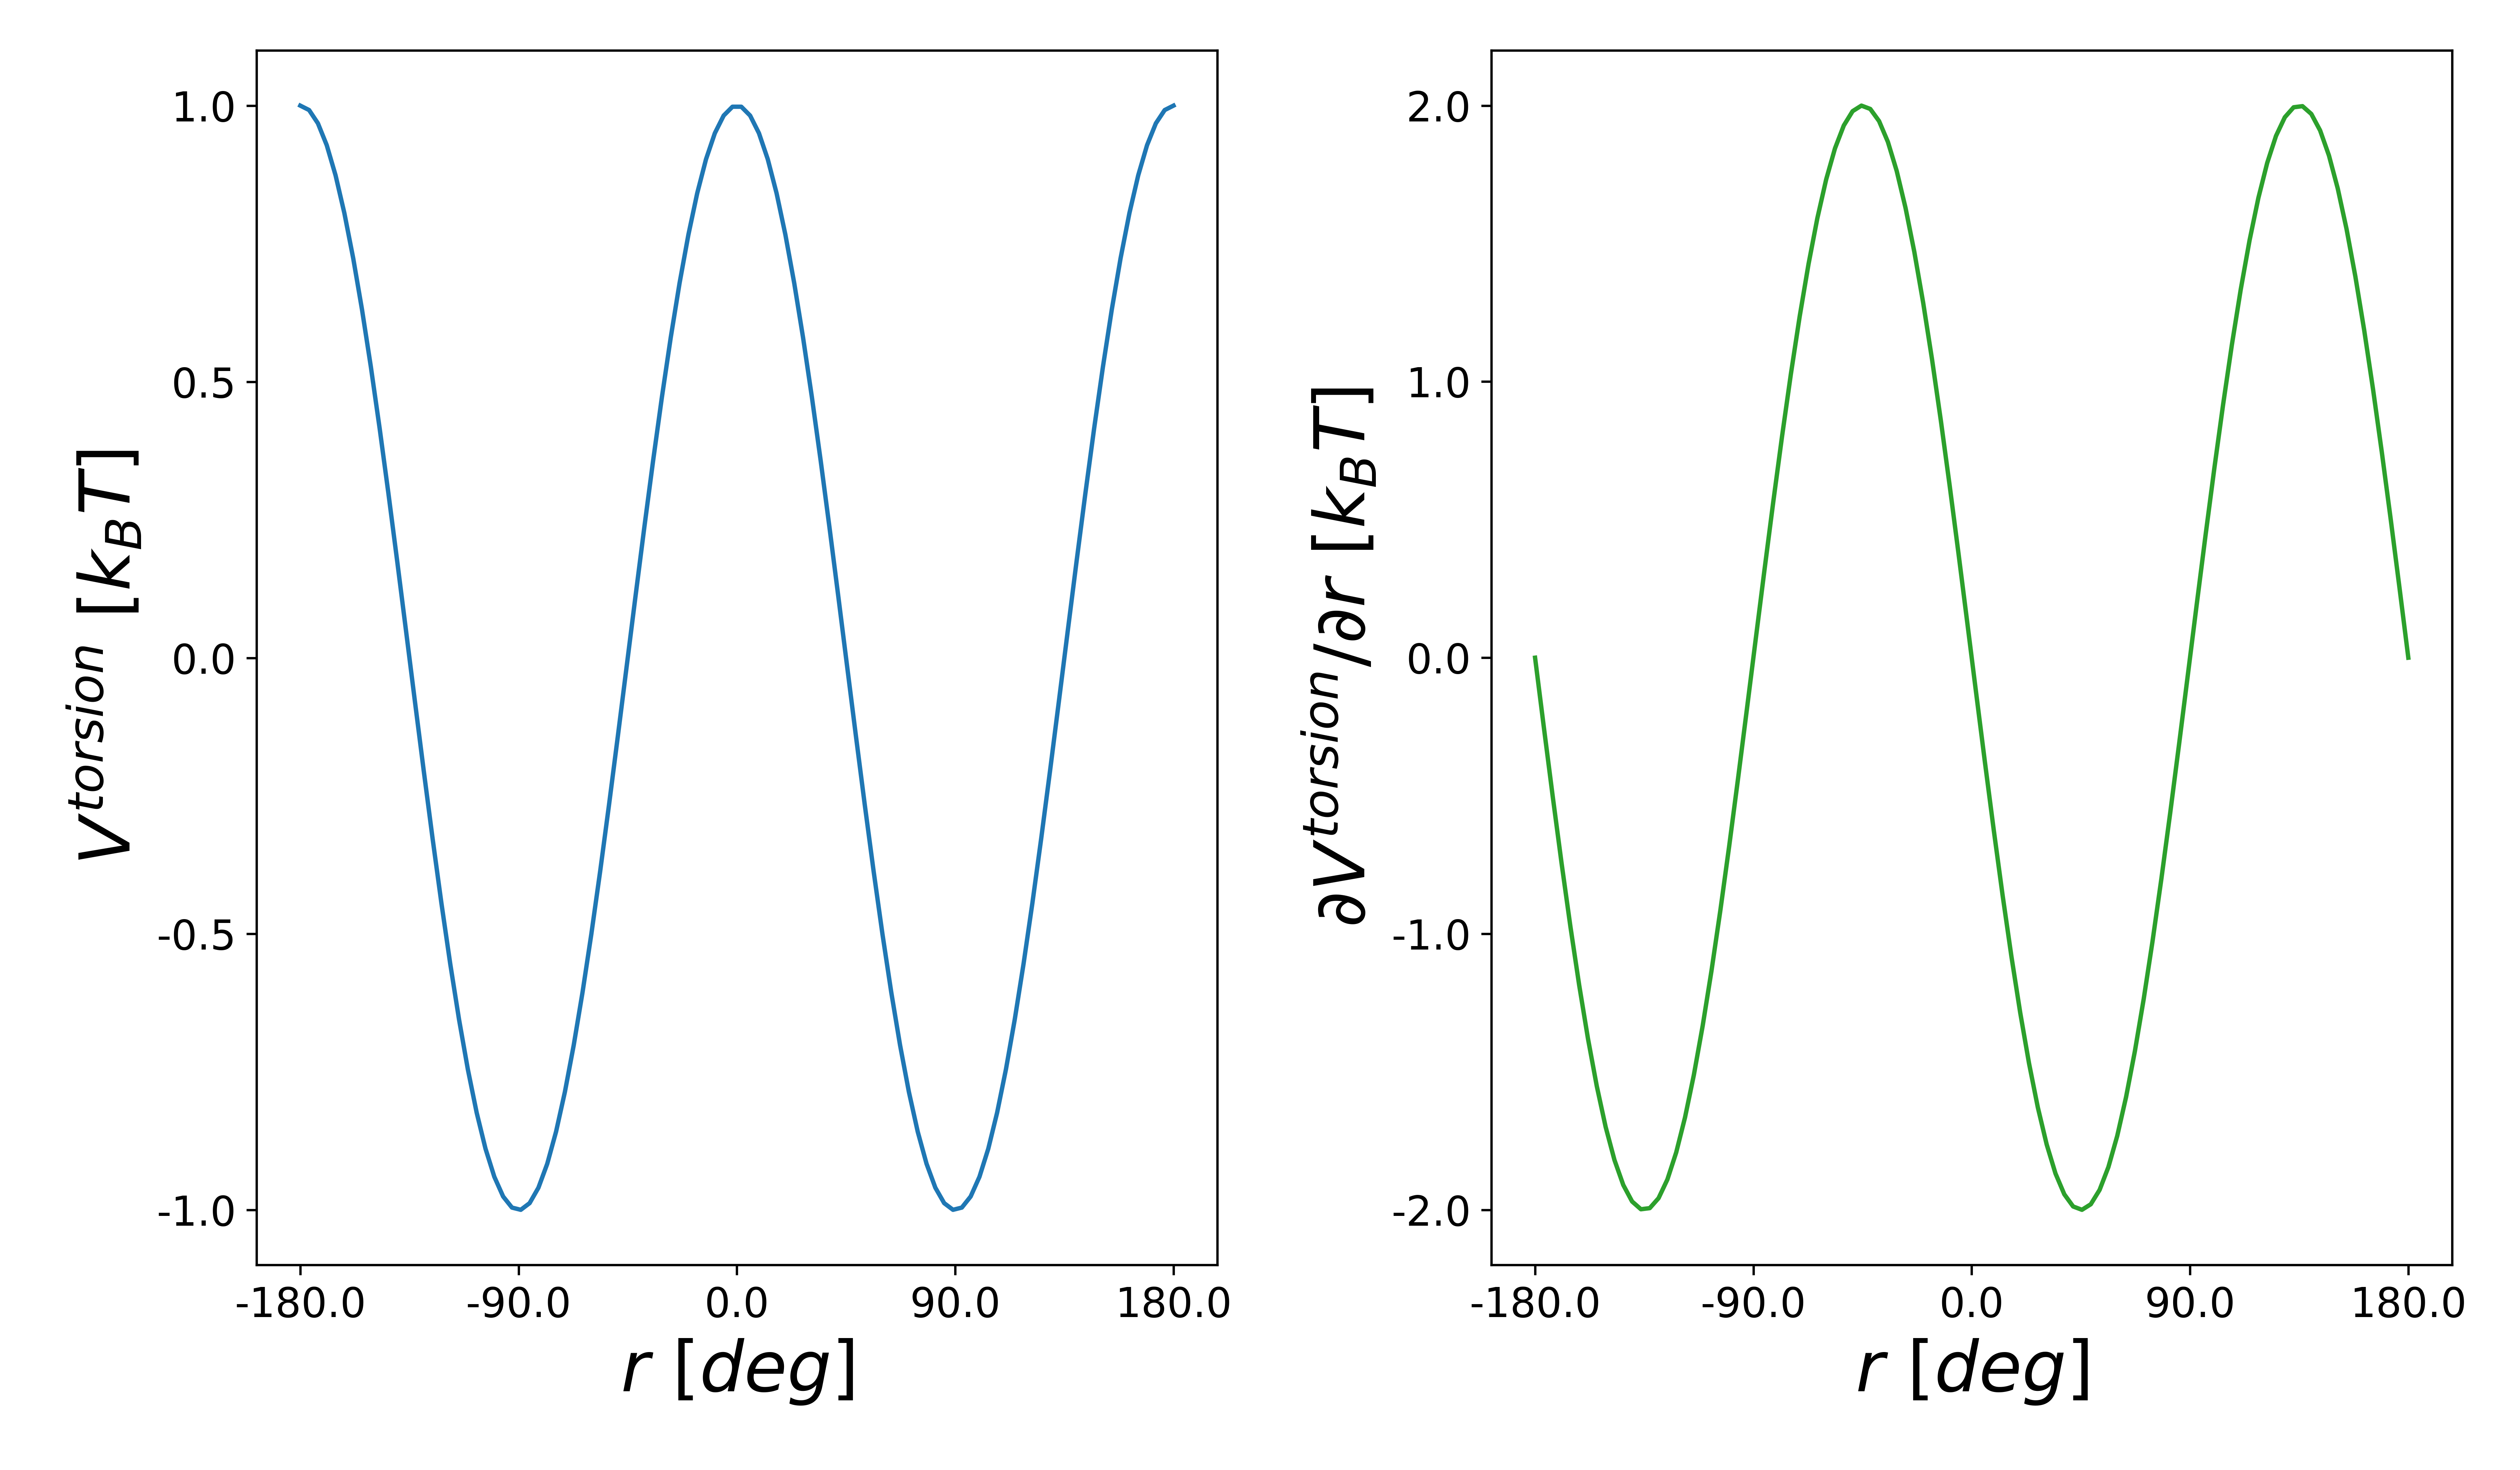
\includegraphics[width=\textwidth]{fig/ForceField/torsion.png}
    \caption{wave Potential is a standard potential used for bond or angle bending in force fields}
    \label{fig:torsion}
\end{figure}
where 

The nonbondeds are split into two subterms.
\begin{equation}
    V^{nonbonded}  = V^{culomb} + V^{VdW} 
\end{equation}

The culombic term describes the interactions of partial charges in the system, 
\begin{equation}
    V^{culomb}  = \frac{q_i q_j}{4 \pi \sigma_0 r_{ijW}}
\end{equation}
\begin{figure}[h]
    \centering
    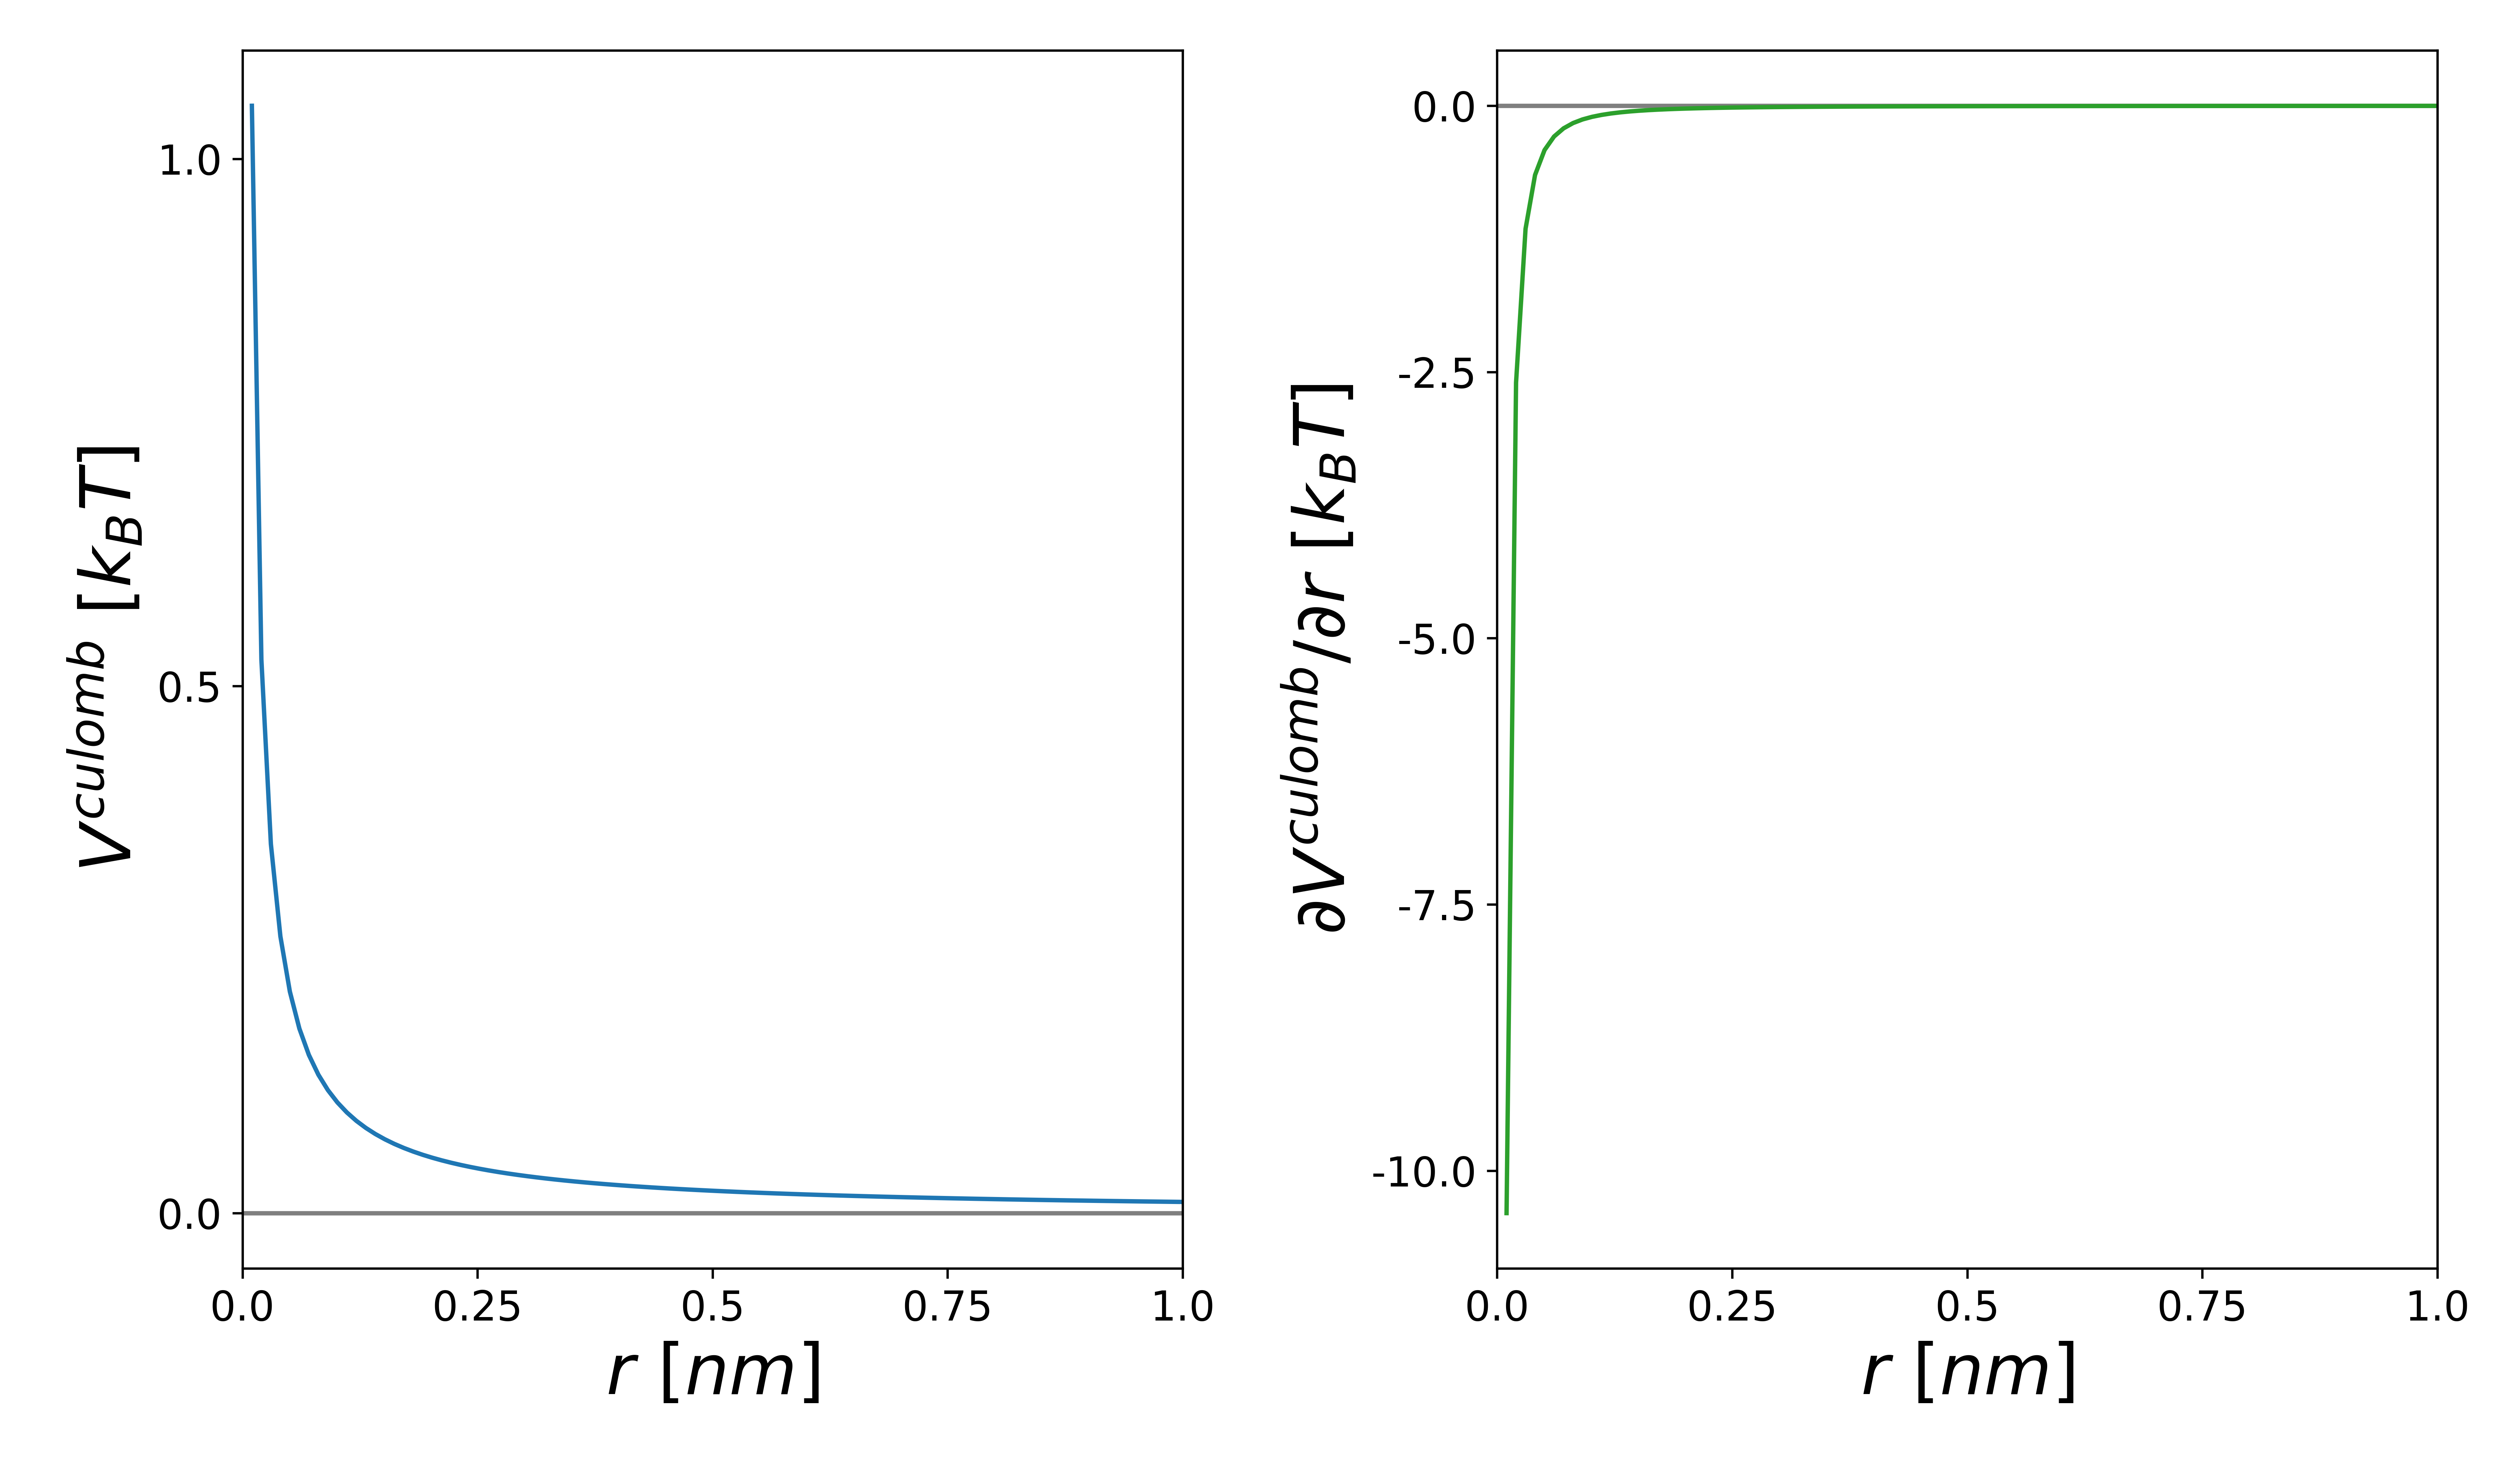
\includegraphics[width=\textwidth]{fig/ForceField/culomb.png}
    \caption{culomb is a standard potential used for bond or angle bending in force fields}
    \label{fig:culomb}
\end{figure}

The Van der Waals term describes ... 
\begin{equation}
    V^{VdW}  = (\frac{C_12}{r^{12}_ij}-\frac{C_6}{r^{6}_ij}) 
\end{equation}
\begin{figure}[h]
    \centering
    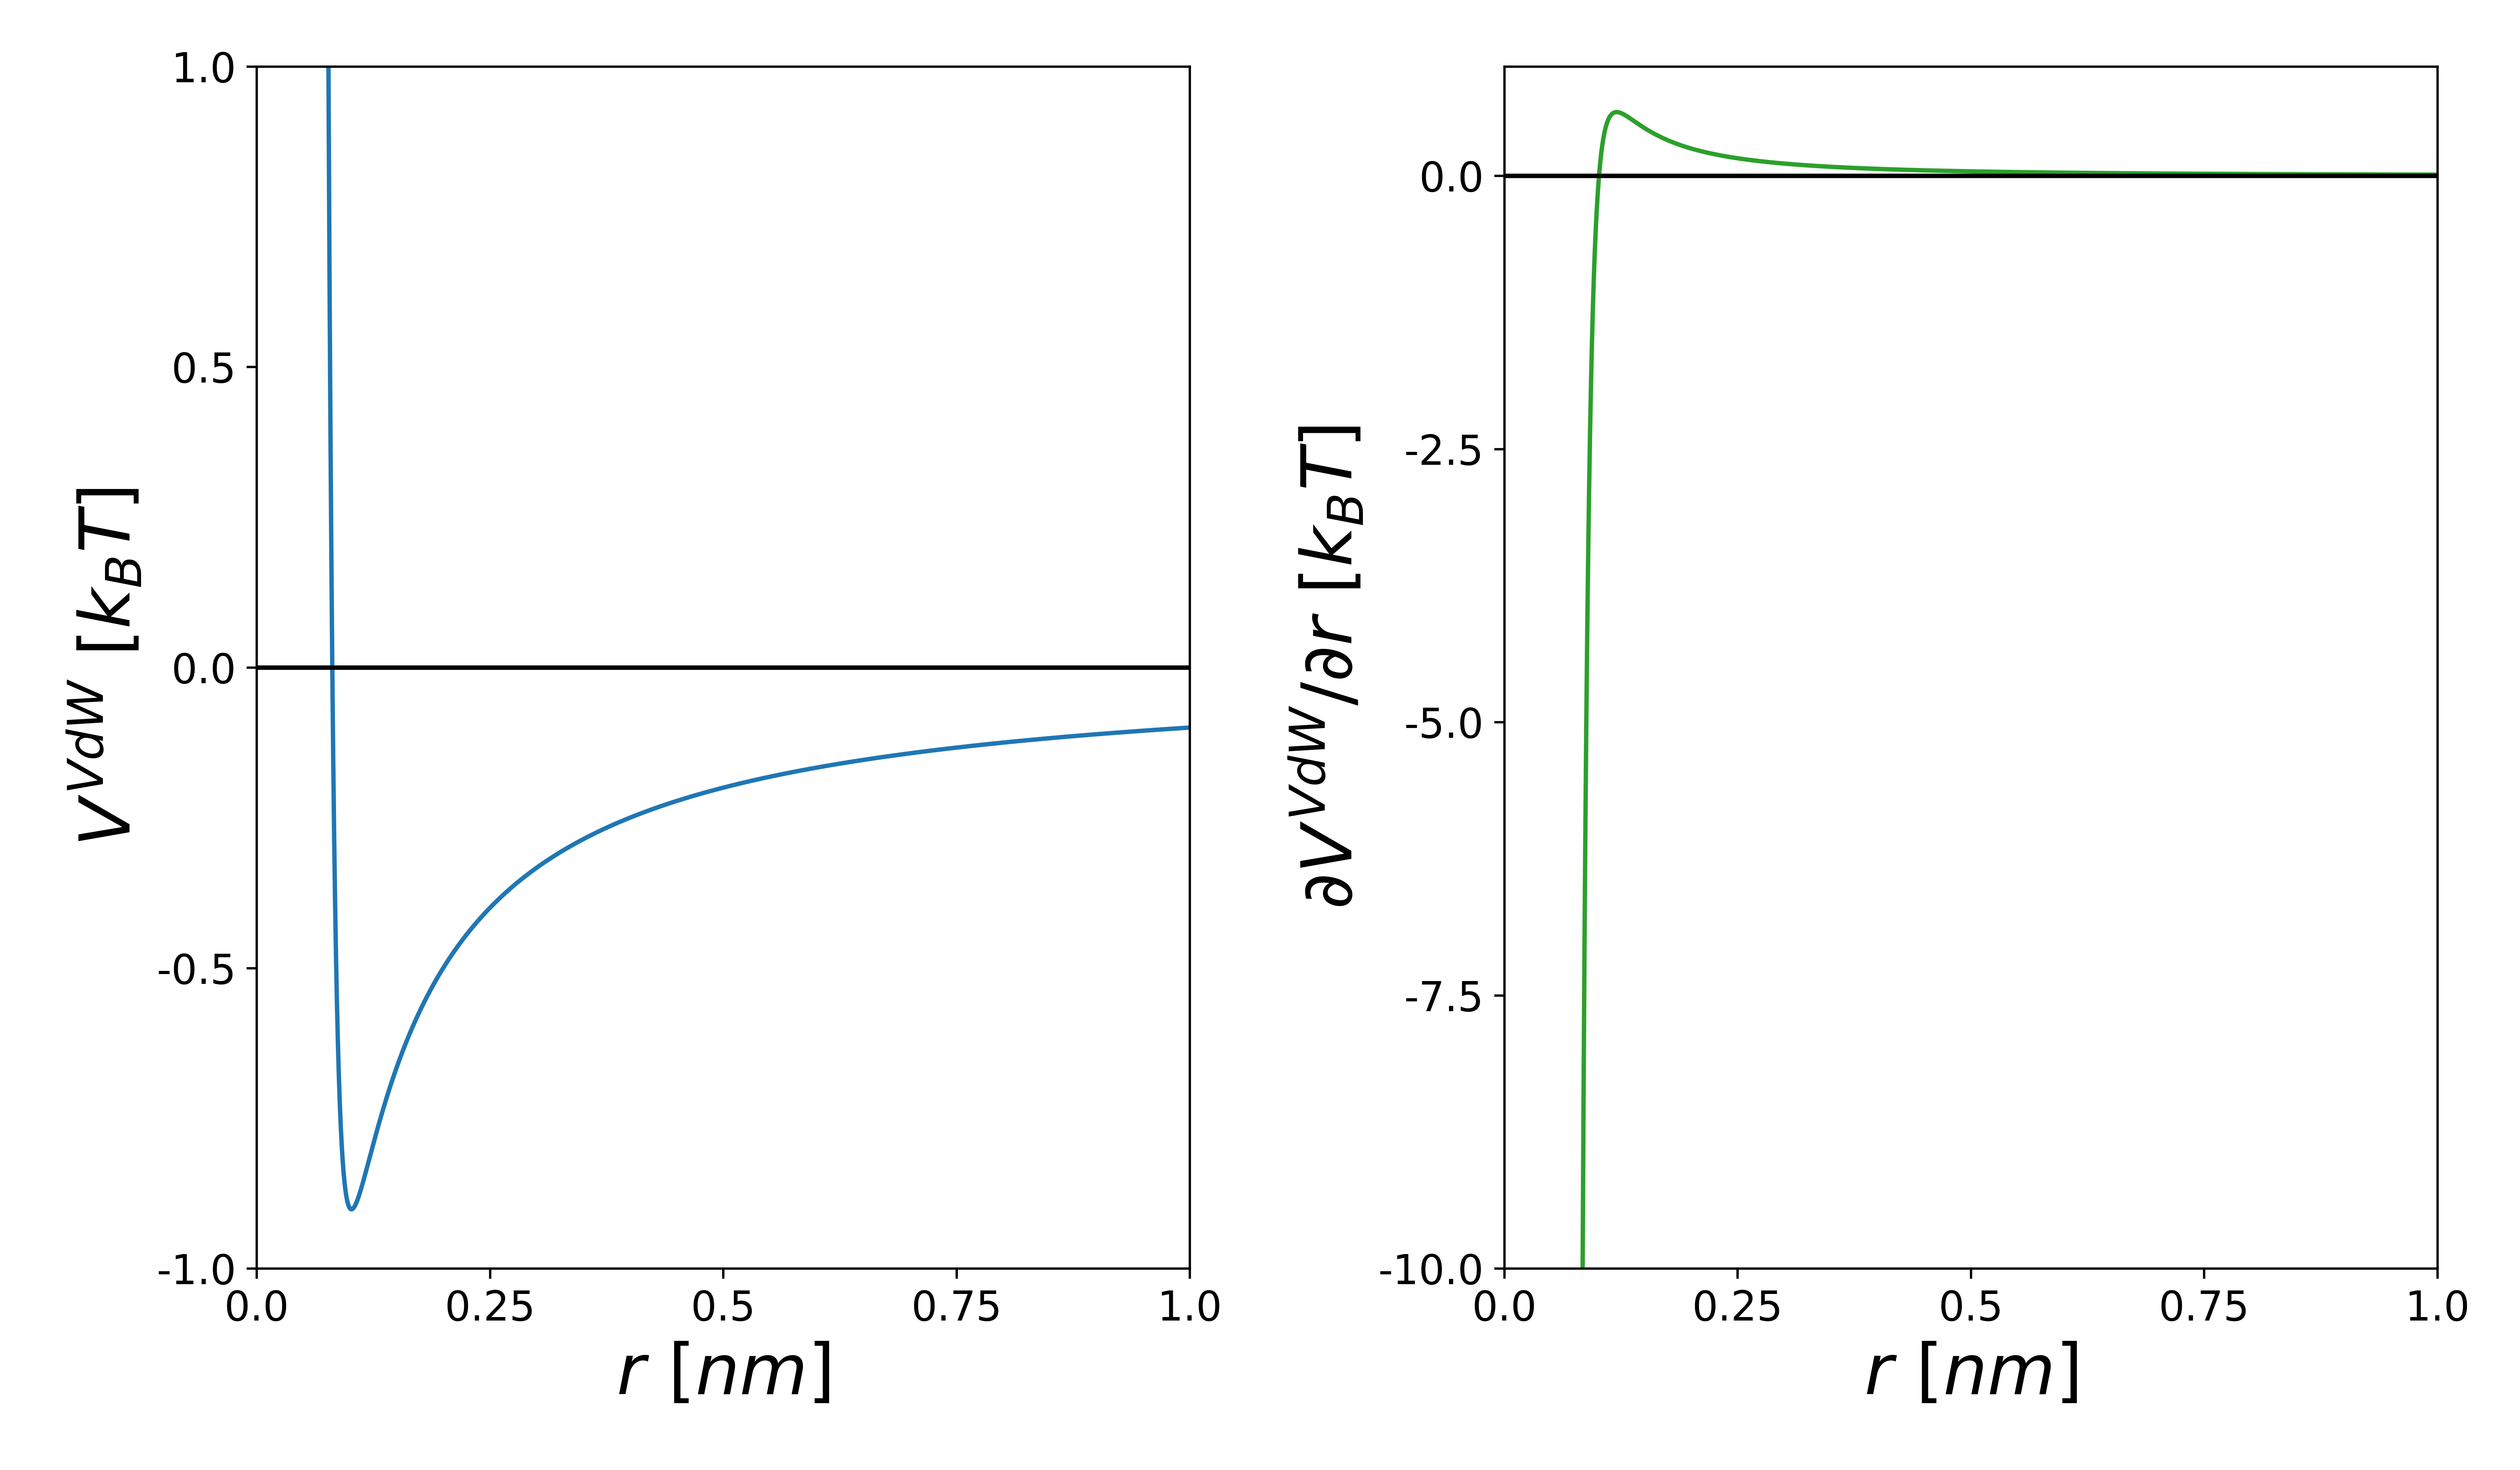
\includegraphics[width=\textwidth]{fig/ForceField/vdw.png}
    \caption{VdW Potential is a standard potential used for bond or angle bending in force fields}
    \label{fig:VdW}
\end{figure}

%%%Integration
\subsection{Integration}
A plethora of different integrators can be used to integrate the force field function. On example is the Metropolis-Monte Carlo integrator, that depends on the Metropolis-Hastings Criterion\cite{Hastings1970},
\begin{equation}
    
\end{equation}

But for MD the most used algorithm is the leap-frog integrator, which integrates the newtonian laws of motion\cite{Newton},
\begin{equation}
    \vec{r}(t+\Delta t)~=~\vec{r}(t)+v(t+\frac{1}{2} t)*\Delta t \\
    \vec{v}(t+\frac{1}{2} \Delta t)~=~\vec{v}(t - \frac{1}{2} \Delta t)+a(t)*\Delta t \\
    \vec{a}(t) = \frac{F(r(t)){m}}
\end{equation}
with $F(r(t))$ as $\partial V/ \partial r$ coming from the force field function.

%%%Conditions
\subsection{Conditions}
Periodic boundary

To sample reliably a configurational space, that is physical meaningful, conditions like the microcanoncial or canonical ensemble is generated. To keep the temperature or pressure constant usually a thermostat or barostat is applied.

In this work the weak coupling thermostat is applied and the berendsen barostat.

--- MORE ---


\section{Enhanced Sampling}
Is one of the huge topics of Simulation techniques. It deals with the problem of low probabilities crossing certain barriers in the potential energy landscape.
In order to speed up the sampling, multiple processes concepts were defined. The first concept is modifying the PES and adds for example a gaussian bias potential to a coordinate (GAM, METADYN, ),  or one can smooth the potential(EDS? hmmm).
The second concept is changing the physical parameters of a simulation, like it is done in H-RE or...
For H-RE many parameters can be exchanged. One for example could be temperature or the other one could be a bond.
Replica exchange was used in this thesis to ...

\section{Free Energy Calculations}
\cite{Barros2022}

\subsection{Build System}


\subsection{Sample System}

\begin{figure}[h]
    \centering
    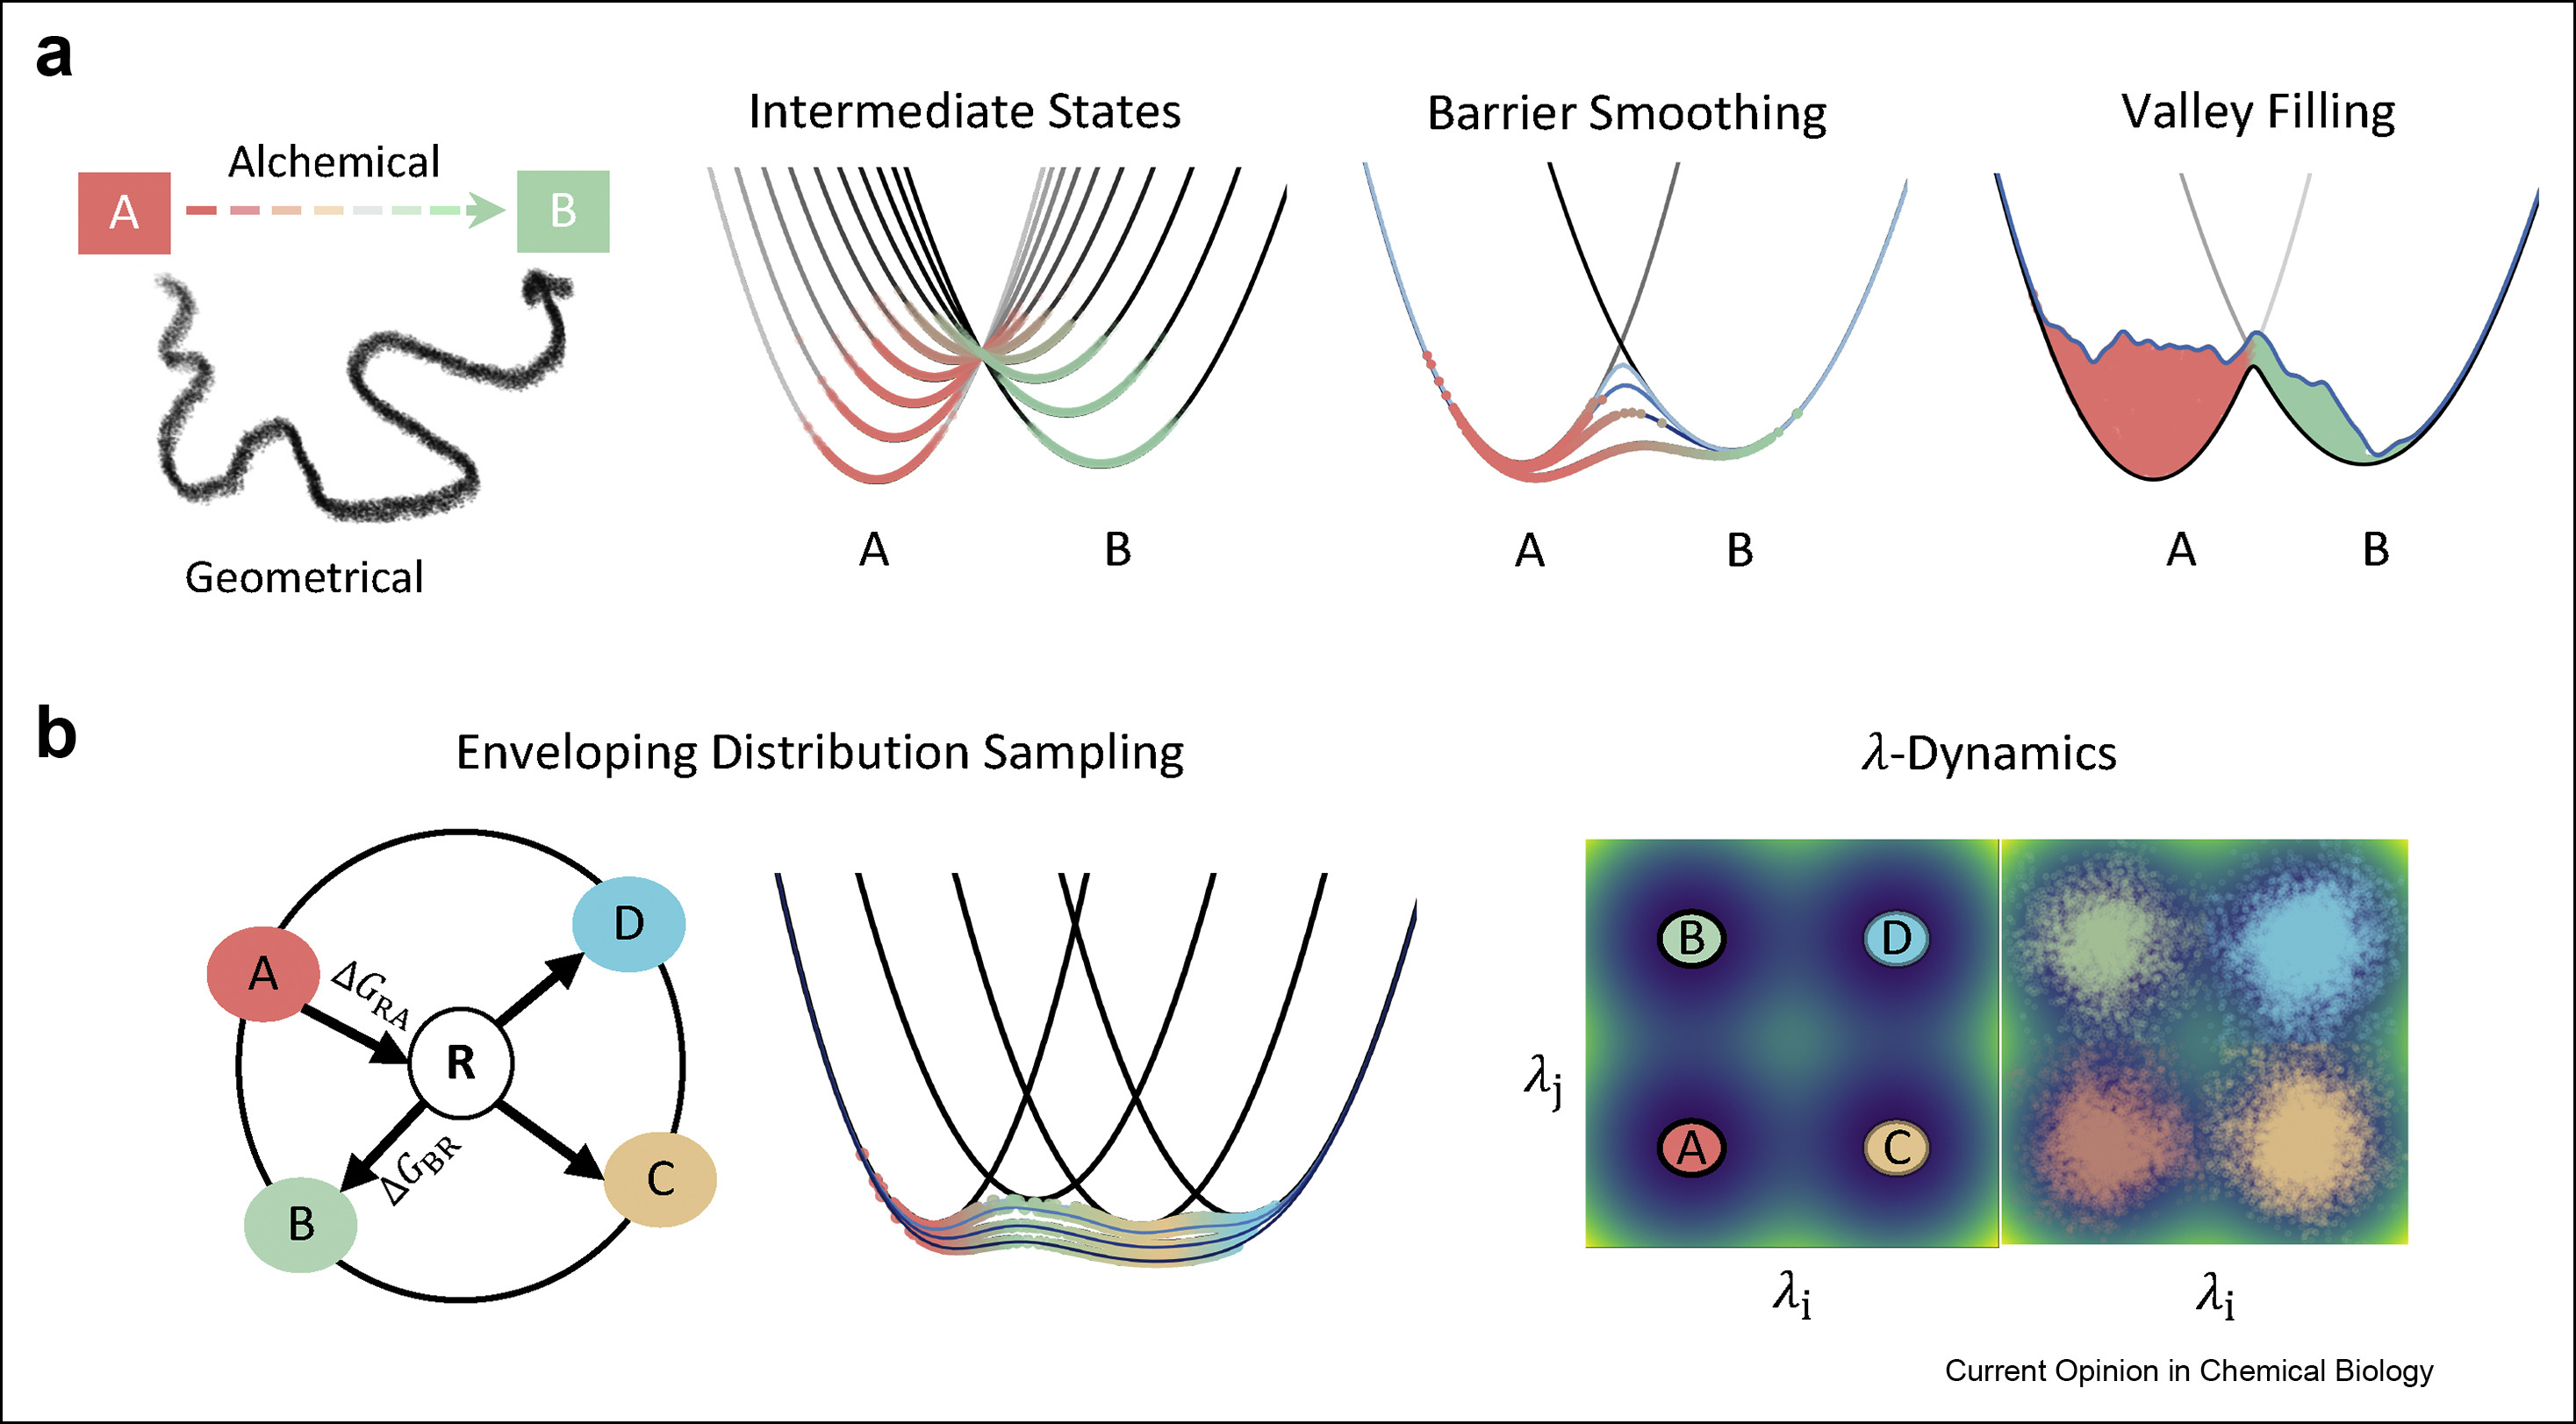
\includegraphics[width=\textwidth]{fig/freeEnergy/samplingMethods.jpg}
    \caption{Ways to sample Free energy systems \cite{Barros2022}}
    \label{fig:my_label}
\end{figure}

\subsubsection{Path Driven Methods}

\subsubsection{Path Free Methods}

\subsubsection{Multistate}



\section{Software Developments in Science}
%Software in Computational

\subsection{Open Source}
% reproducibility, sharebility

\subsection{Demands}
% fast usage, etc

